% !TEX root = ../../buch.tex
% problemstellung.tex -- Beispiel-File für die Beschreibung des Problems
%
% (c) 2020 Prof Dr Andreas Müller, Hochschule Rapperswil
%
\section{Resultate
\label{burgers:section:results}}
\rhead{Resultate}

	Im Folgenden werden die Berechnungen f\"ur eine normalverteilte Startbedingung mit der expliziten und impliziten Methode gezeigt.
	Um den Vergleich zwischen den verschiedenen Methoden besser ersichtlich zu machen, werden die Resultate in zwei Dimensionen aufgezeigt.
	F\"ur jeden Zeitschritt wurde ein neuer Subplot gezeichnet.

	\subsection{Explizit}

	Beim expliziten Verfahren werden die beiden linearen Varianten aufgezeigt,
	wobei sich nur der gew\"ahlte Punkt f\"ur die Multiplikation unterscheidet.
	In \autoref{burgers:fig:ex} zeigen sich die Unterschiede, welche durch die \"Anderung des gewählten Punktes für die Multiplikation hervorgerufen werden.


    \begin{figure}
	\centering
	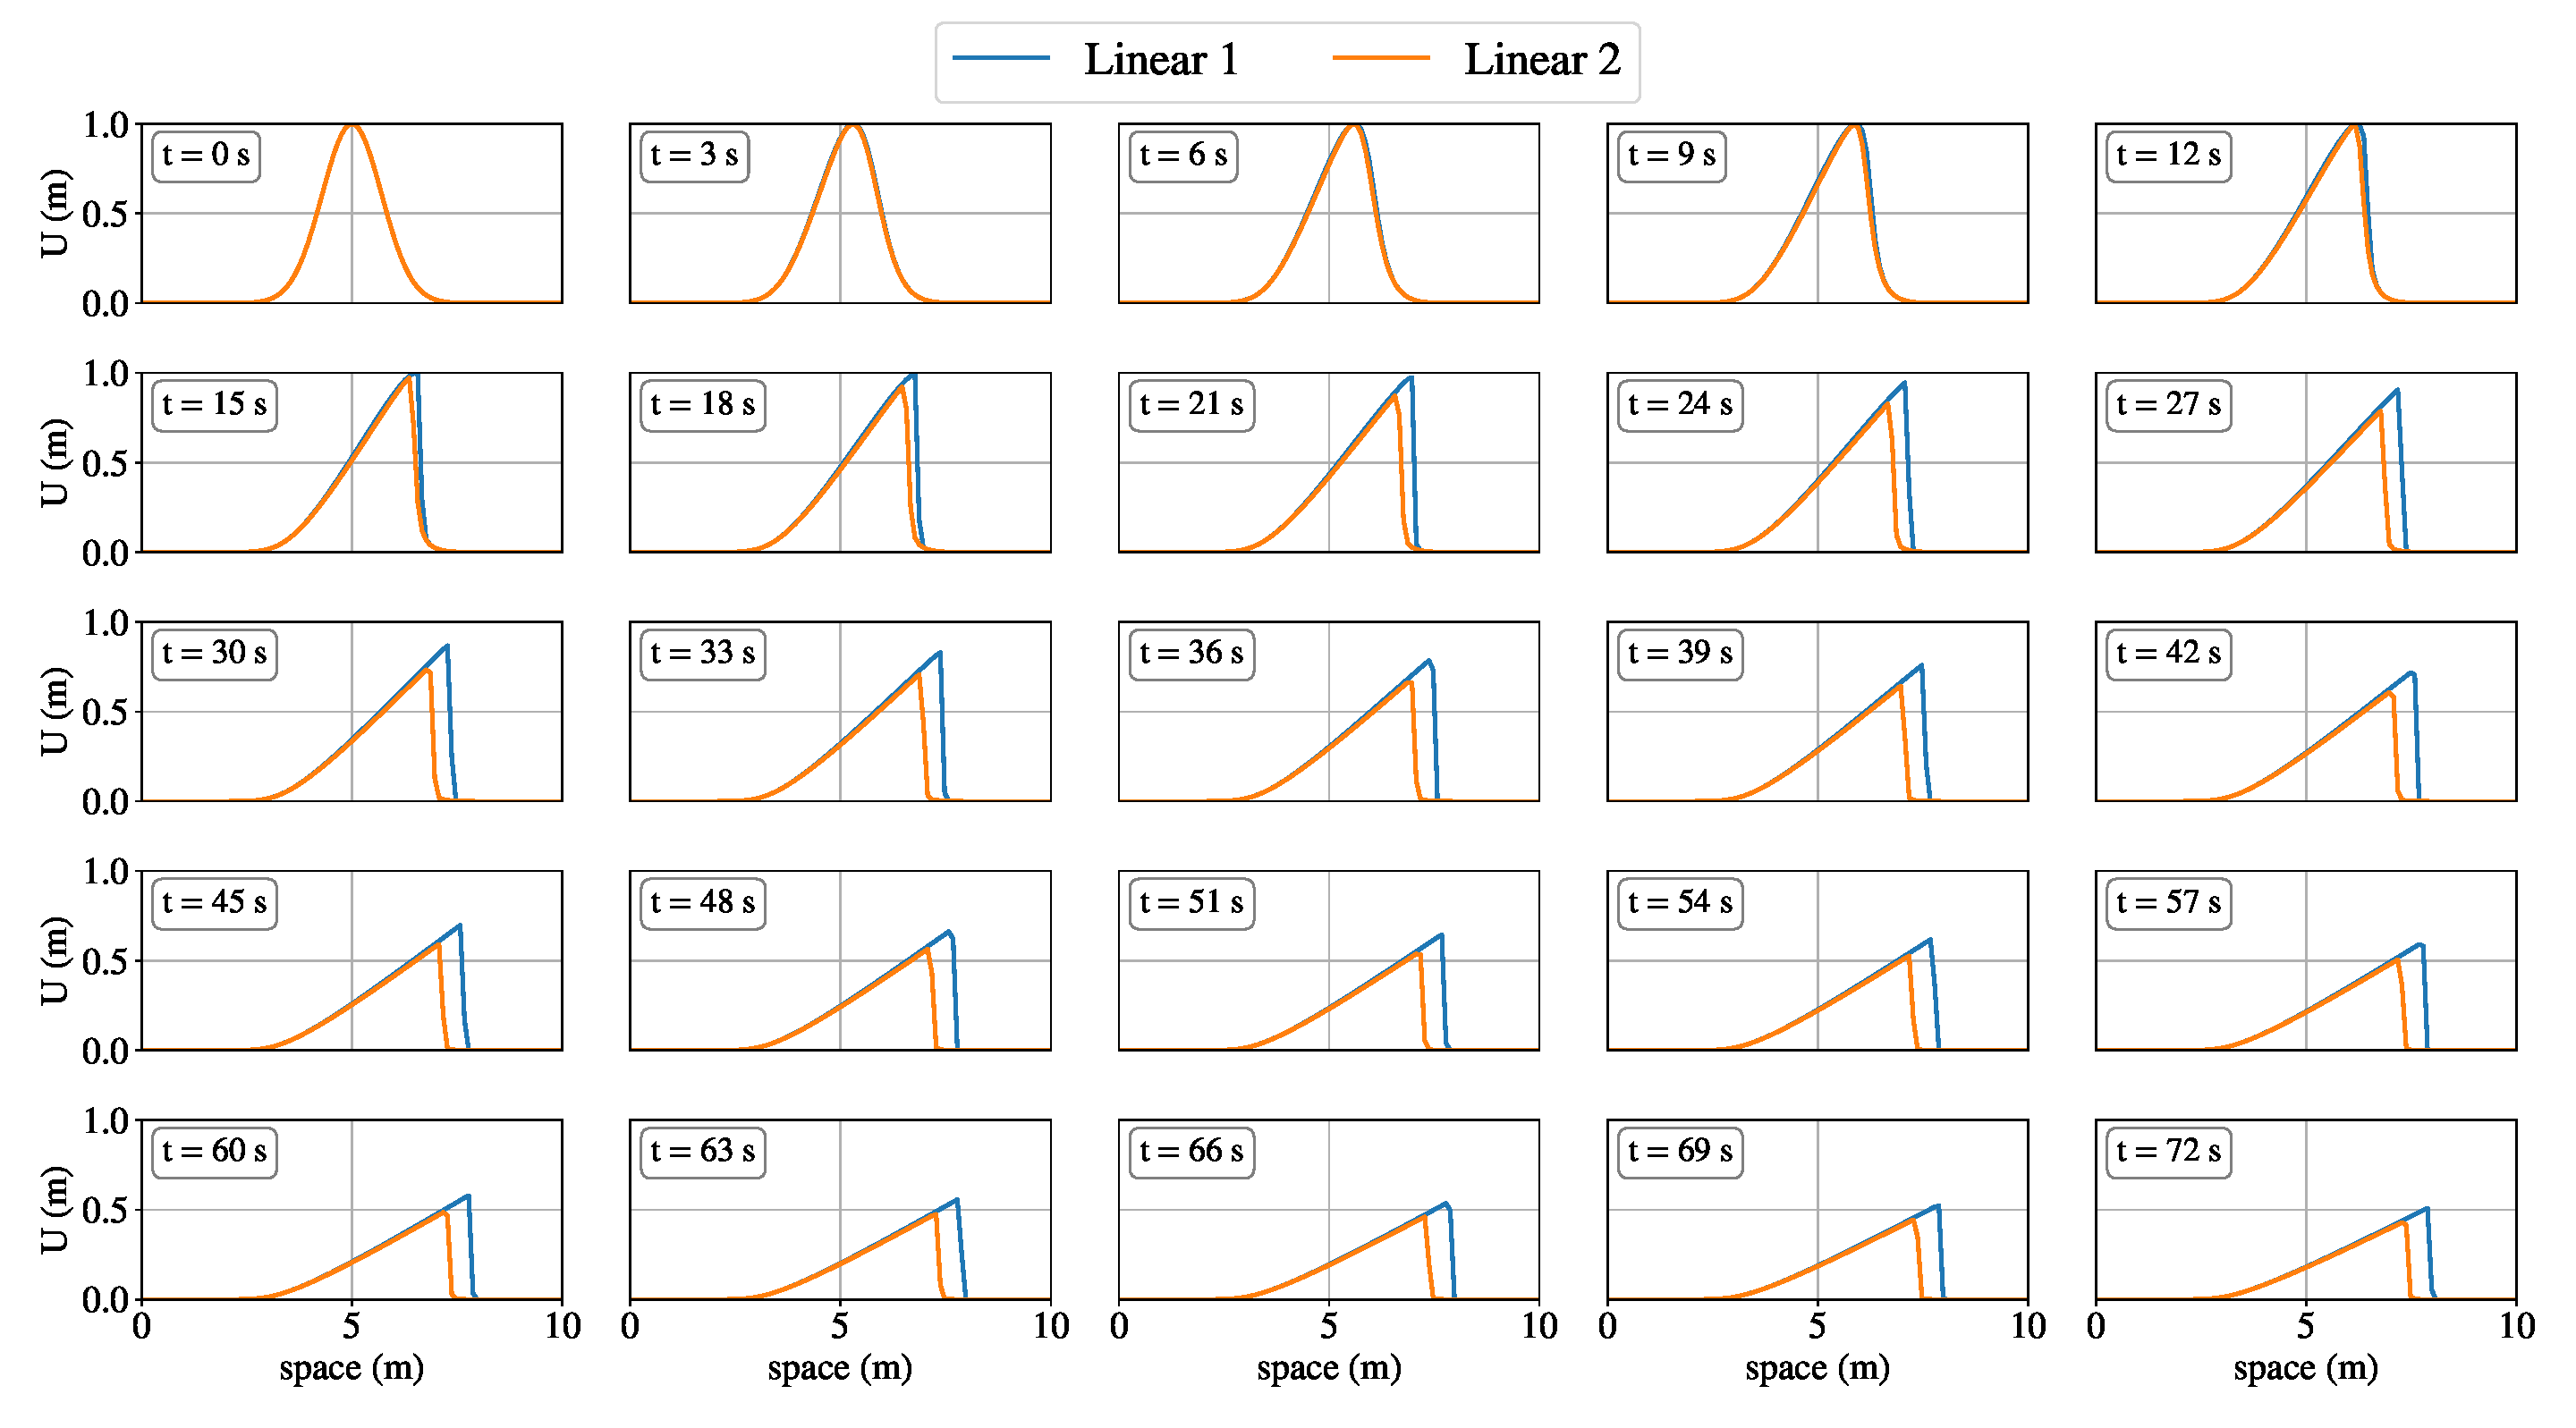
\includegraphics[width=1\textwidth]{papers/burgers/BurgersEquation/lin_paper.pdf}
	\caption{L\"osung Explizit}
	\label{burgers:fig:ex}
	\end{figure}

	\subsubsection{Robert-Asselin-Time-Filter}
	In \autoref{burgers:fig:time} kann die L\"osung mit dem beschriebenen Tiefpass-Filters aus Abschnitt \ref{burgers:sec:cm} entnommen werden.
	Wird der D\"ampfungsfaktor $\alpha$ zu gross gew\"ahlt, wird die L\"osung zu stark gefiltert.

	  \begin{figure}
		\centering
		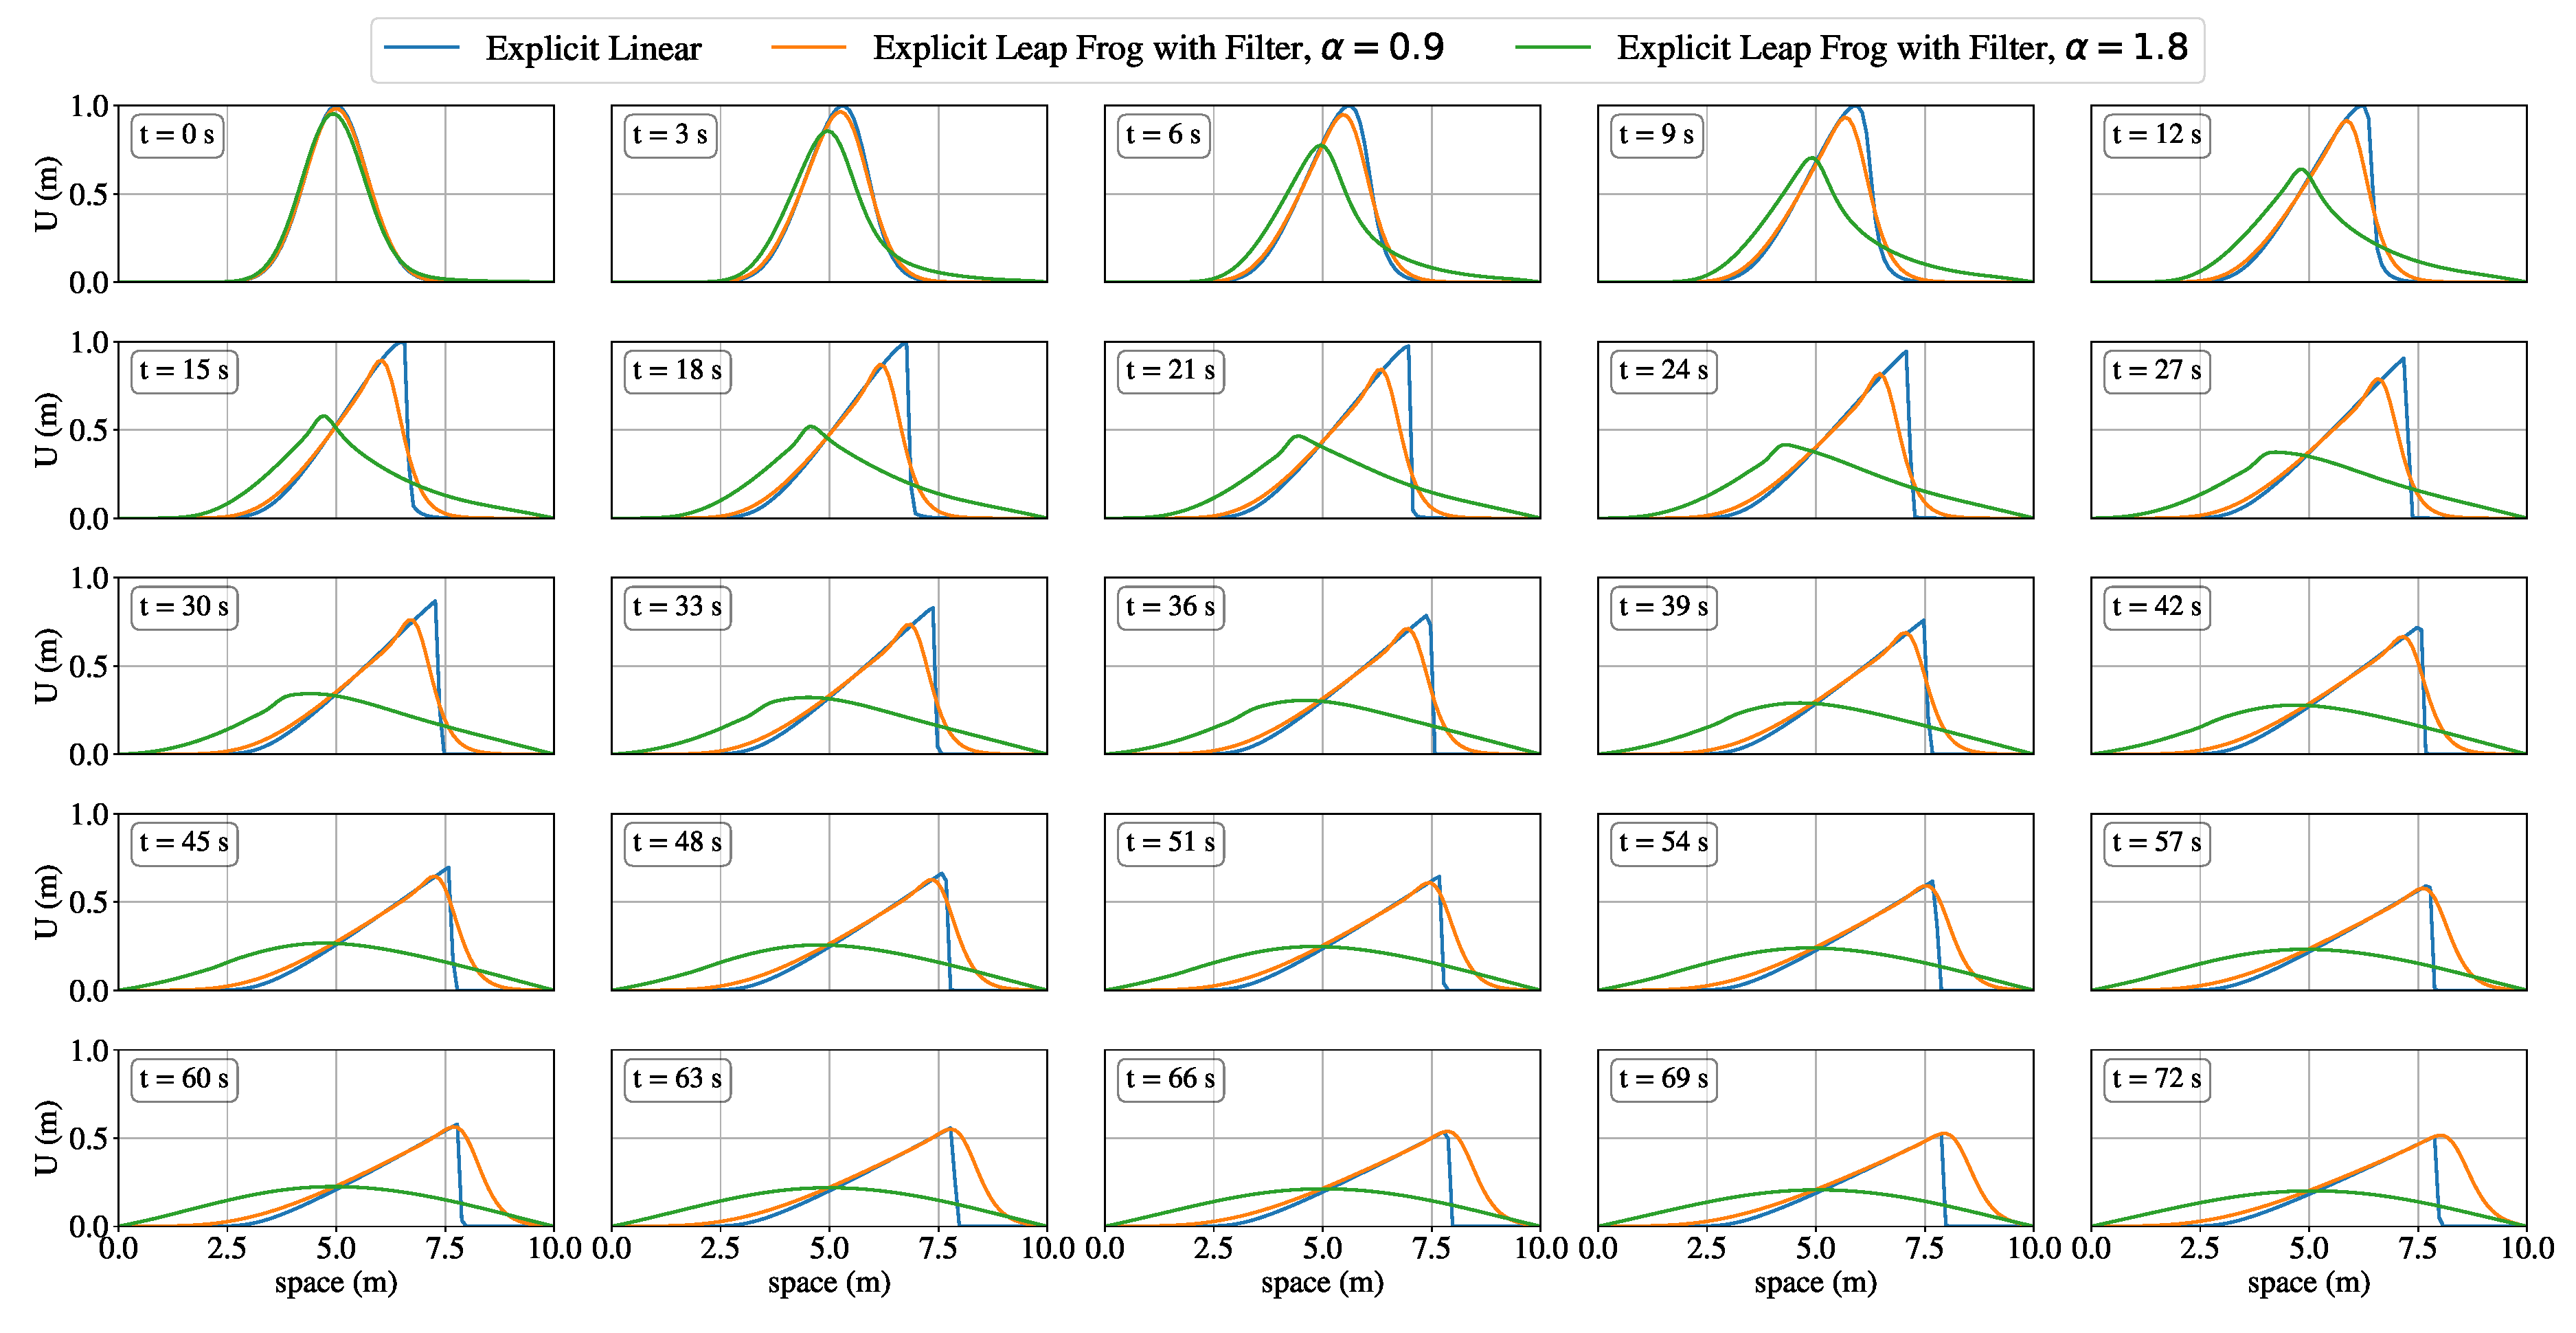
\includegraphics[width=1\textwidth]{papers/burgers/BurgersEquation/time_filter.pdf}
		\caption{L\"osung Explizit mit linearem und Leap-Frog Ansatz, Tiefpassfilterung der Leap-Frog L\"osung }
		\label{burgers:fig:time}
		\end{figure}


	\subsection{Implizit}

	Die Unterschiede bei den impliziten Verfahren sind in \autoref{burgers:fig:imp} etwas besser ersichtlich.
	Es zeigt, dass der gew\"ahlte Punkt f\"ur die Ableitung bei der Leap-Frog Methode einen gr\"osseren Einfluss hat.
	Die Welle ist etwas tr\"ager, als die der L\"osung der quadratischen und linearen impliziten Varianten.

    \begin{figure}
	\centering
	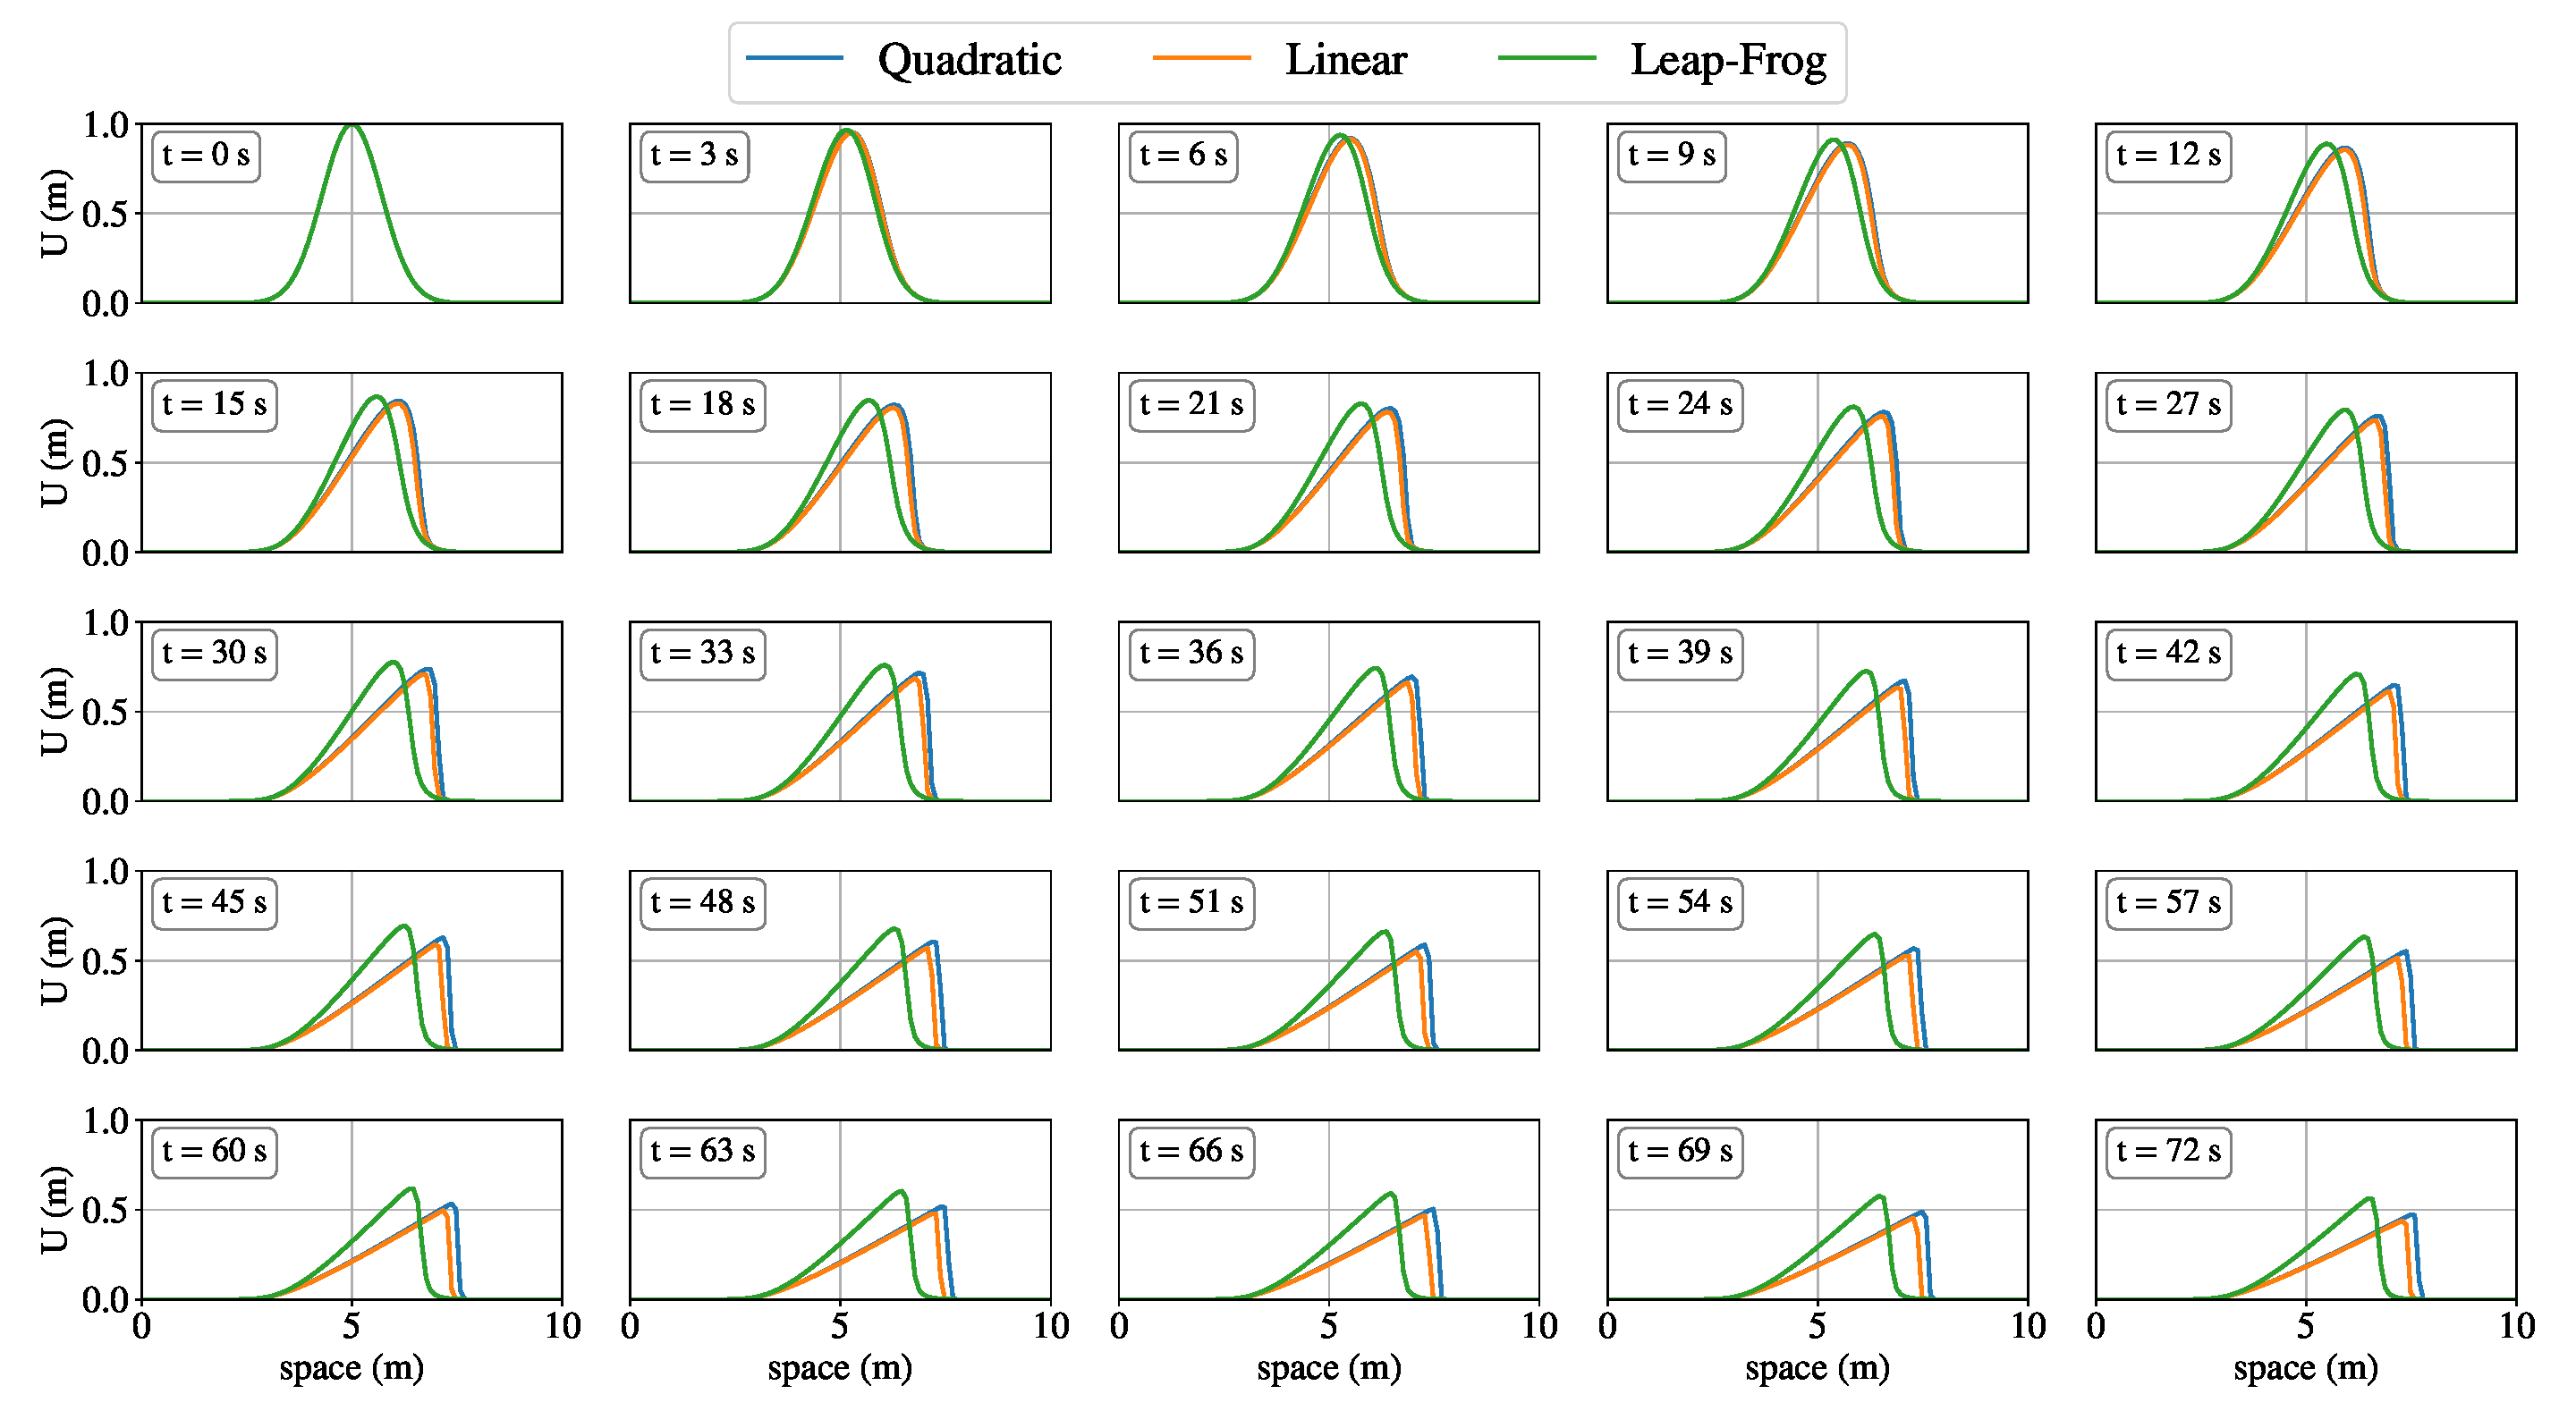
\includegraphics[width=1\textwidth]{papers/burgers/BurgersEquation/imp_paper.pdf}
	\caption{L\"osung Implizit}
	\label{burgers:fig:imp}
	\end{figure}

\newpage %Literaturverzeichnis wäre vor der letzten Abbildung
